\section{Related Works}

\begin{frame}{Taxonomy of Related Works}
    \begin{figure}
        \centering
        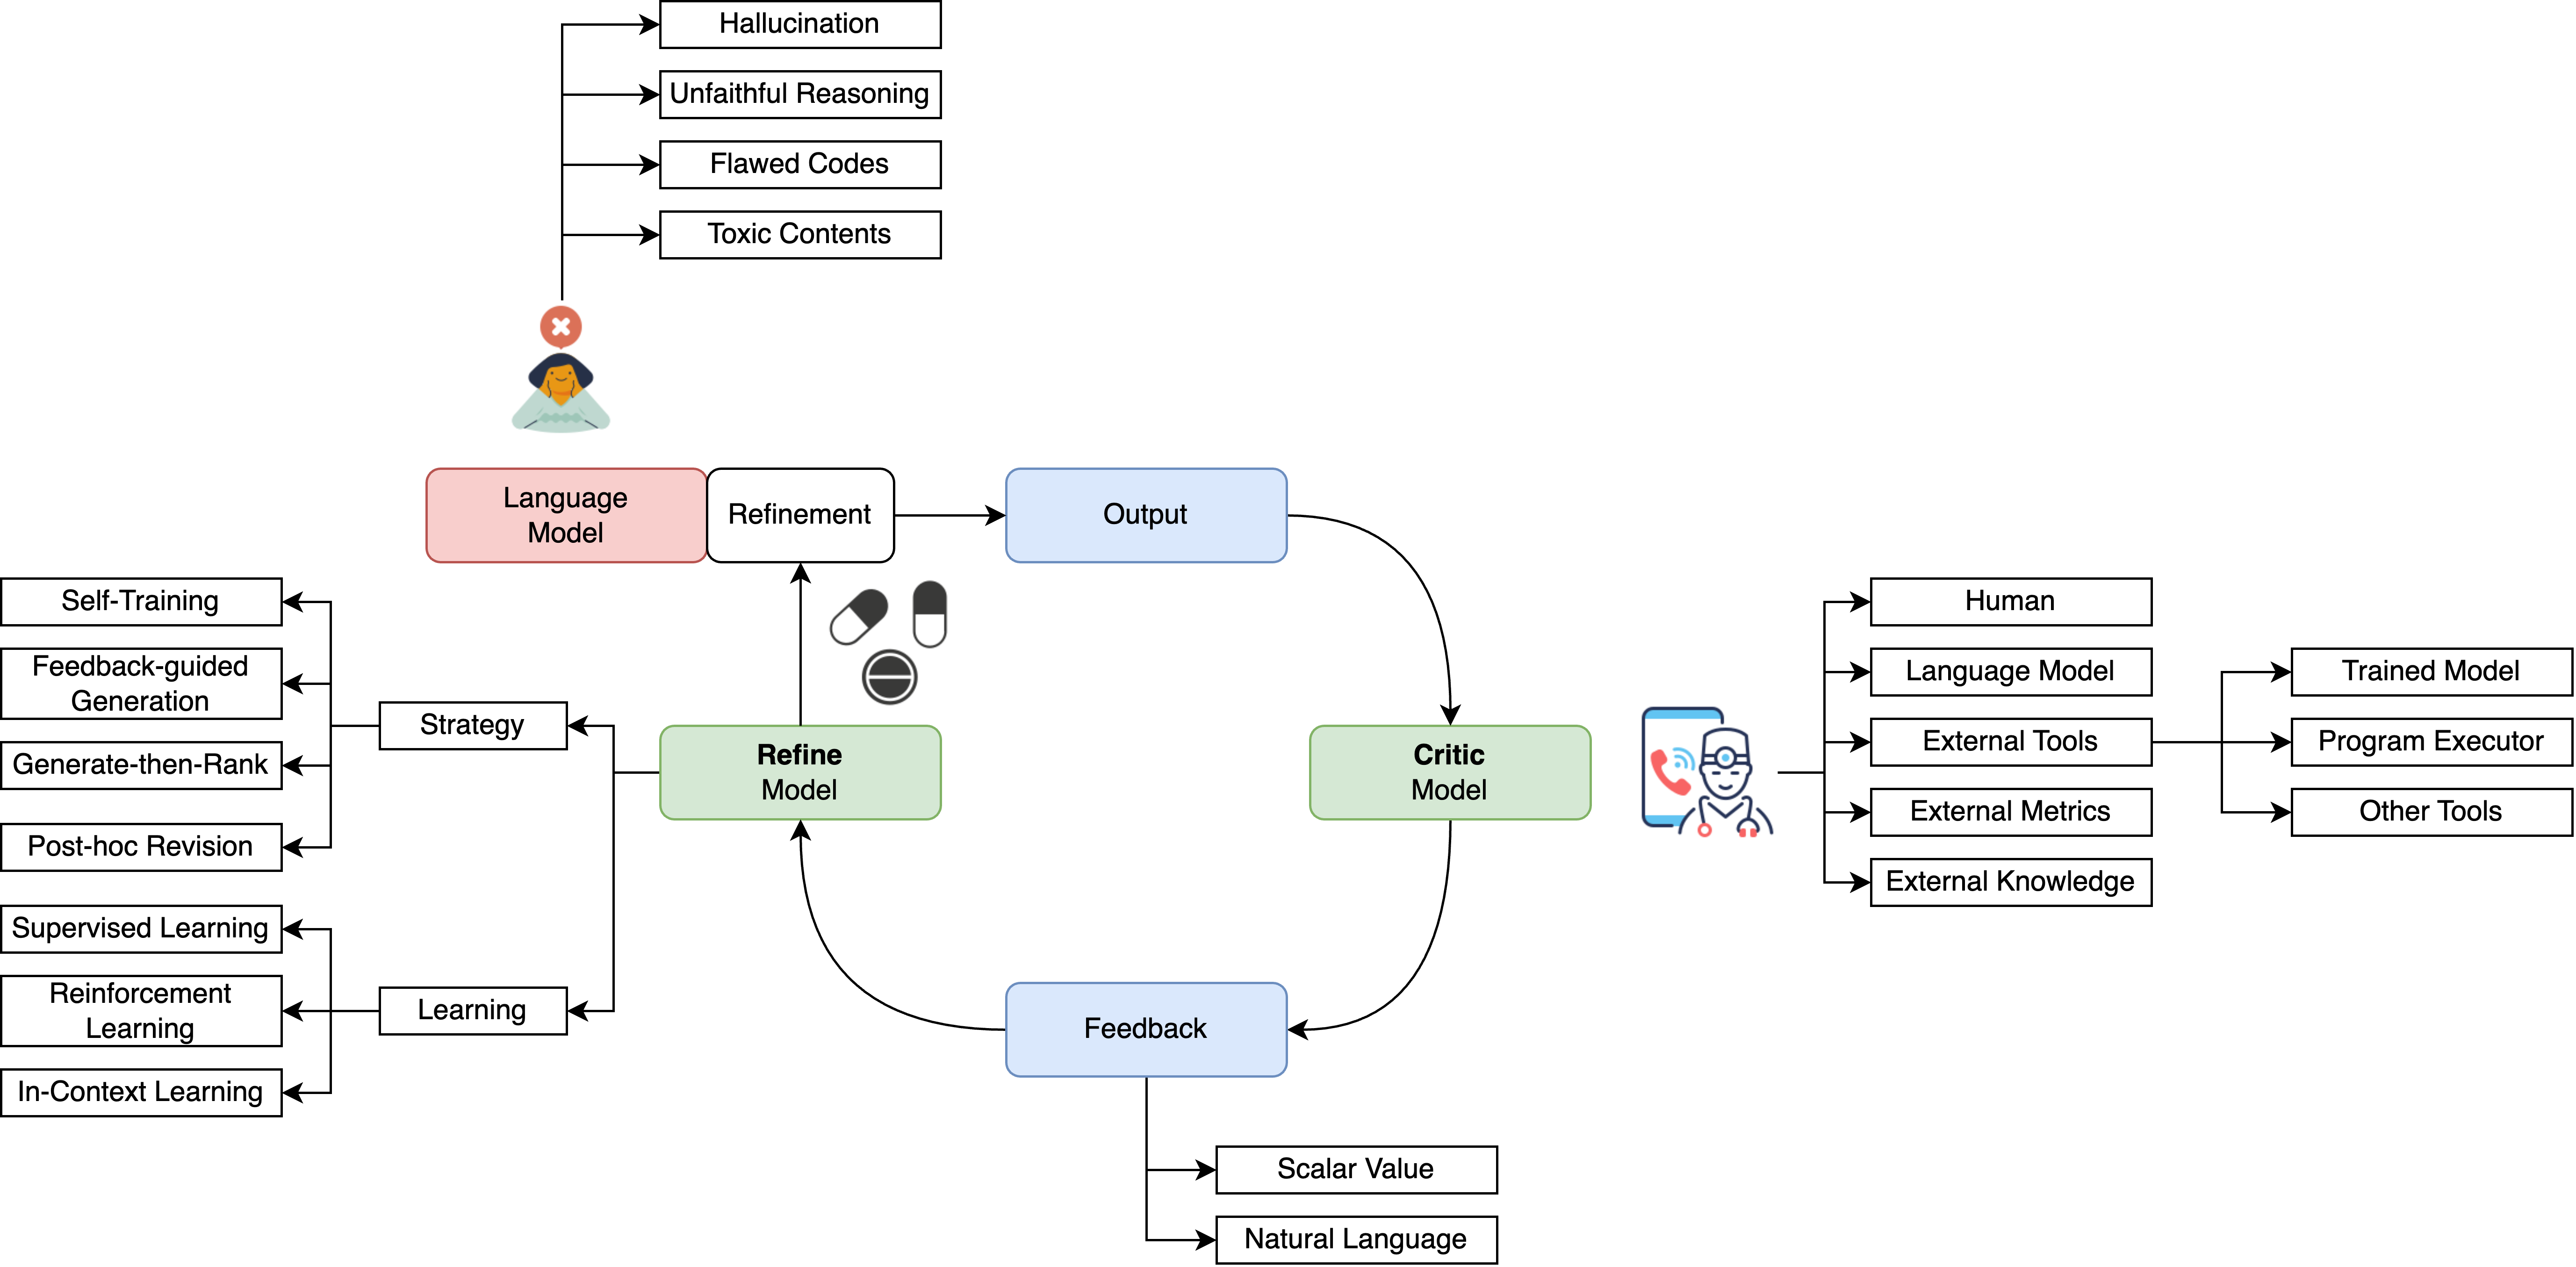
\includegraphics[width=1\textwidth]{img/taxonomy}
        \captionsetup{font=small,labelformat=empty}
        \caption{Taxonomy of works on self-correcting LLMs.}\label{fig:taxonomy}
    \end{figure}
\end{frame}

\begin{frame}{Refine Model}
    The Refine Model is the most active area of research in the field. Existing works can be classified based on the following key questions:
    \begin{enumerate}
        \item Need to update the LLMs?
              \begin{itemize}
                  \item Yes: Self-Training~\cite{huang2022large}, Supervised Learning~\cite{bai2022training}, Reinforcement Learning~\cite{dubois2024alpacafarm}.
                  \item No: In-Context Learning~\cite{dong2022survey}.
              \end{itemize}

        \item When to refine: generation-time or post-hoc?
              \begin{itemize}
                  \item Generation-time: Generate-then-Rank~\cite{cobbe2021training}, Feedback-Guided Generation~\cite{yao2023tree}.
                  \item Post-hoc: Models/Tools as Feedback~\cite{zhang2023selfedit}, Multi-Agent Debate~\cite{du2023improving}.
              \end{itemize}
    \end{enumerate}
\end{frame}

\begin{frame}{Obstacles and Prospects}
    \begin{enumerate}
        \item Obstacle: Predominantly, existing LLMs, like OpenAI's GPT-4, are proprietary. Alternatively, they may possess an impractically vast number of parameters for training within the confines of this study, as seen in the 70-billion parameter Llama model.

        \item Prospect: A number of notable studies have been conducted on the utilization of self-correcting LLMs in autonomous code correction. Examples include Google Deepmind's SelfDebug~\cite{chen2023teaching} and Shanghai Jiao Tong University's SelfEvolve~\cite{jiang2023selfevolve}.
    \end{enumerate}
\end{frame}

\begin{frame}{Research Direction}
    \begin{figure}[!htb]
        \centering
        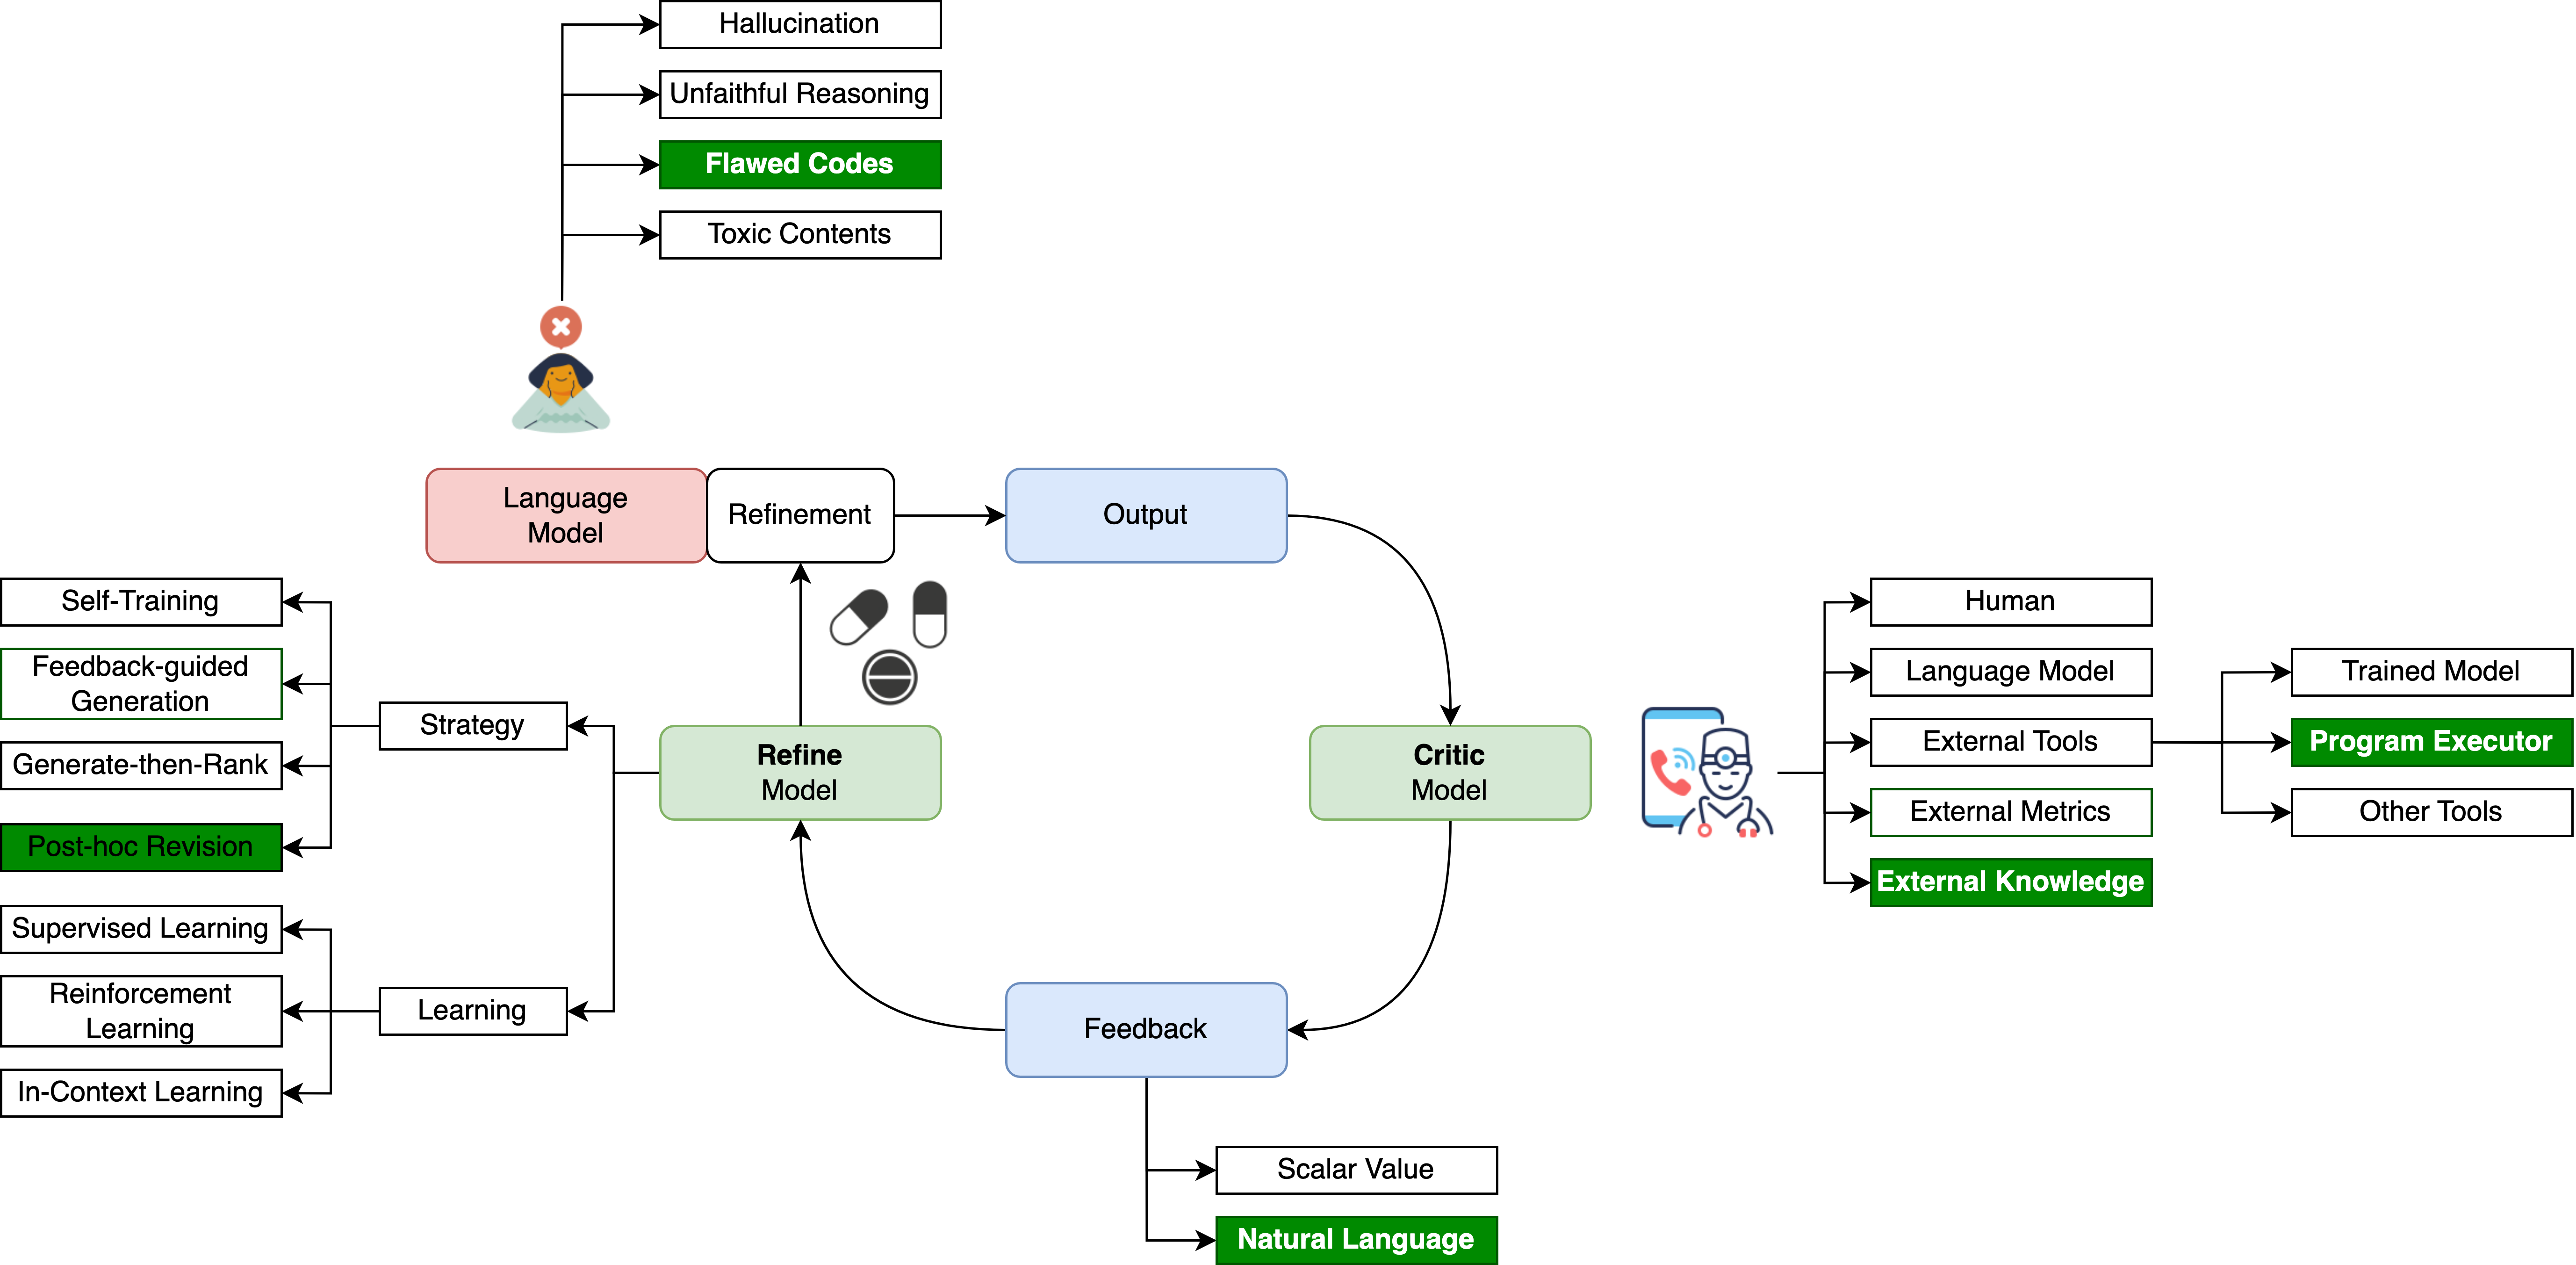
\includegraphics[width=1\textwidth]{img/direction_of_research}
        \captionsetup{font=small,labelformat=empty}
        \caption{Research Direction.}
    \end{figure}
\end{frame}
